
C++源码的编译过程很简单:

\begin{lstlisting}[style=styleCXX]
// chapter-01/01-hello/hello.cpp

#include <iostream>
int main() {
	std::cout << "Hello World!" << std::endl;
	return 0;
}
\end{lstlisting}

现在,要获得可执行文件,只需要运行一个命令。用文件名作为参数使用编译器:

\begin{tcblisting}{commandshell={}}
$ g++ hello.cpp -o a.out
\end{tcblisting}

代码正确,因此编译器将生成一个机器可以理解的二进制文件。可以通过文件名来运行程序:

\begin{tcblisting}{commandshell={}}
$ ./a.out
Hello World!
$
\end{tcblisting}

然而,随着项目的增长,无法将所有内容都保存在一个文件中。务实的代码实践建议,文件应该较小,并采用组织良好的结构,并且手动编译每个文件是一个令人厌烦和脆弱的过程。

\subsubsubsection{1.2.1\hspace{0.2cm}CMake?}

假设通过编写一个遍历项目树,并编译所有内容的脚本来自动化构建。为了避免不必要的编译,脚本将检测源码(脚本)是否修改过。现在,我们希望有一种方法来管理传递给每个文件编译器的参数——最好是可配置的。此外,脚本应该知道如何链接已编译的文件,或者构建整个解决方案,以便在更大的项目中重用或作为模块。

添加的特性越多,就越有可能得到一个成熟的解决方案。构建软件是一个通用的过程(其中有一些步骤可以跳过):

\begin{itemize}
\item 
编译可执行程序和库

\item 
管理依赖关系

\item 
测试

\item 
安装

\item 
打包

\item 
生成文档

\item 
测试更多功能
\end{itemize}

要做出一个真正模块化的、功能强大的C++构建应用来满足各种需求很难,但CMake确实做到了。Kitware的Bill Hoffman在20多年前实现了CMake的第一个版本,现在有了更多的功能,并得到了社区的支持。目前,CMake的开发很活跃,并已成为C和C++开发人员的行业标准。

以自动化的方式构建代码的问题比CMake出现的要早得多,所以会有很多选择:Make、Autotools、SCons、Ninja、Premake等。但为什么CMake可以后来居上呢?

关于CMake,有几件事我觉得(主观地说)很重要:

\begin{itemize}
\item 
专注于支持现代编译器和工具链。

\item 
CMake是真正的跨平台——支持Windows、Linux、macOS和Cygwin的构建。

\item 
为主流IDE生成项目文件:Microsoft Visual Studio, Xcode和Eclipse CDT。此外,也是其他项目的模型,如CLion。

\item 
CMake操作在合适的抽象级别上——允许将文件分组到可重用的目标和项目中。

\item 
有很多用CMake构建的项目,其提供了一种简单的方法将它们包含到自己的项目中。

\item 
CMake将测试、打包和安装视为构建过程的固有组成。

\item 
弃用旧的、未使用的特性,从而保持CMake的精简。
\end{itemize}

CMake提供了统一的、流线型的体验。不管是在IDE中构建,还是直接从命令行构建,还照顾到构建后阶段。即使前面所有的环境都不同,持续集成/持续部署(CI/CD)流水也可以轻松地使用相同的CMake配置,并使用单一标准构建项目。

\subsubsubsection{1.2.2\hspace{0.2cm}如何工作?}

可能会有这样的印象:CMake是在一端读取源代码,在另一端生成二进制文件的工具——虽然原则上没问题,但这并不是全部。

CMake自己不能构建任何东西——它依赖于系统中的其他工具来执行实际的编译、链接和其他任务。可以将它看作是构建过程的协调器,知道需要完成哪些步骤,最终目标是什么,以及如何为工作找到合适的工人和材料。

这个过程有三个阶段:

\begin{itemize}
\item 
配置

\item 
生成

\item 
构建
\end{itemize}

\hspace*{\fill} \\ %插入空行
\noindent
\textbf{配置阶段}

这个阶段会读取存储在源码树目录中的项目信息,并为生成阶段准备输出目录或构建树。CMake首先创建一个空的构建树,并收集工作环境的信息,例如:架构、编译器、链接器和存档打包器。此外,还要检查编译器是否能编译简单的测试程序。

接下来,执行CMakeLists.txt项目配置文件(CMake项目是用CMake的编码语言配置的)。这个文件是CMake项目的基础部分(源文件可以稍后添加),它告诉CMake有关项目结构、目标和依赖项(库和其他CMake包)的信息。此过程中,CMake将收集的信息存储在构建树中,例如:系统详细信息、项目配置、日志和临时文件,这些信息将用于下一阶段,会创建一个CMakeCache.txt文件来存储变量(例如编译器和其他工具的路径),节省下次配置期间的时间开销。

\hspace*{\fill} \\ %插入空行
\noindent
\textbf{生成阶段}

读取项目配置之后,CMake将为当前工作环境生成一个构建系统。构建系统只是其他构建工具的简化配置文件(例如,GNU Make或Ninja的Makefiles和Visual Studio的IDE项目文件),CMake仍然可以通过生成器表达式对构建配置应用进行一些修改。

\begin{tcolorbox}[colback=blue!5!white,colframe=blue!75!black,title=Note]
生成阶段在配置阶段之后自动执行,在提到构建系统的“配置”或“生成”时,本书和其他资源经常提到这两个阶段。要显式地分段运行配置阶段,可以使用cmake-gui。
\end{tcolorbox}

\hspace*{\fill} \\ %插入空行
\noindent
\textbf{构建阶段}

为了生成项目中指定的工件,必须运行适当的构建工具。可以通过IDE直接调用,也可以使用CMake命令行。这些构建工具都会执行构建步骤,使用编译器、链接器、静态和动态分析工具、测试框架、报告工具,以及其他工具来生成目标。

这个解决方案的美妙之处在于,能够用单一配置(即相同的项目文件)为每个平台按需生成构建系统:

\begin{center}
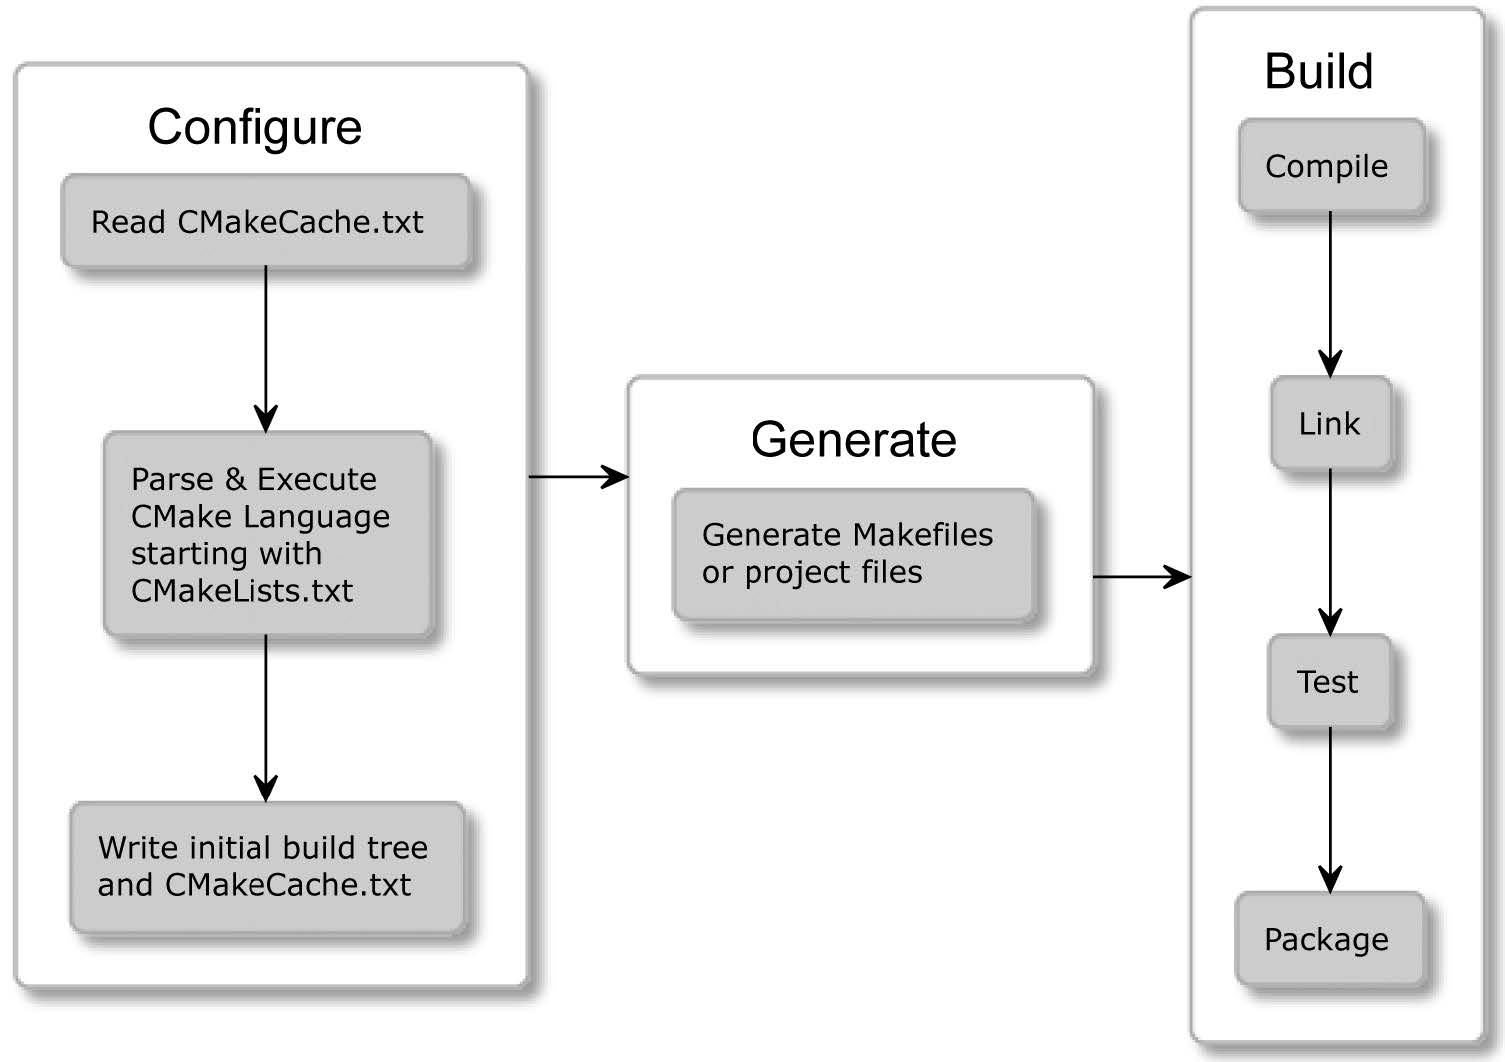
\includegraphics[width=0.9\textwidth]{content/1/chapter1/images/1.jpg}\\
图1.1  CMake的各个阶段
\end{center}

还记得hello.cpp吗?CMake可以很容易的对其进行构建。所需要的就是下面的CMakeLists.txt文件和两个简单的命令,\texttt{cmake -B buildtree}和\texttt{cmake -{}-build buildtree}:

\begin{lstlisting}[style=styleCMake]
# chapter01/01-hello/CMakeLists.txt: Hello world in the CMake language
	
cmake_minimum_required(VERSION 3.20
project(Hello)
add_executable(Hello hello.cpp)
\end{lstlisting}

下面是Dockerized Linux系统的输出:

\begin{tcblisting}{commandshell={}}
root@5f81fe44c9bd:/root/examples/chapter01/01-hello# cmake
-B buildtree.
-- The C compiler identification is GNU 9.3.0
-- The CXX compiler identification is GNU 9.3.0
-- Check for working C compiler: /usr/bin/cc
-- Check for working C compiler: /usr/bin/cc -- works
-- Detecting C compiler ABI info
-- Detecting C compiler ABI info - done
-- Detecting C compile features
-- Detecting C compile features - done
-- Check for working CXX compiler: /usr/bin/c++
-- Check for working CXX compiler: /usr/bin/c++ -- works
-- Detecting CXX compiler ABI info
-- Detecting CXX compiler ABI info - done
-- Detecting CXX compile features
-- Detecting CXX compile features - done
-- Configuring done
-- Generating done
-- Build files have been written to: /root/examples/
chapter01/01-hello/buildtree
root@5f81fe44c9bd:/root/examples/chapter01/01-hello# cmake
--build buildtree/
Scanning dependencies of target Hello
[ 50%] Building CXX object CMakeFiles/Hello.dir/hello.cpp.o
[100%] Linking CXX executable Hello
[100%] Built target Hello
\end{tcblisting}

运行:

\begin{tcblisting}{commandshell={}}
root@68c249f65ce2:~# ./buildtree/Hello
Hello World!
\end{tcblisting}

我们生成了一个在buildtree目录中的构建系统。执行构建阶段,并生成能够运行的最终二进制文件。

现在了解了最终结果的样子,我相信你会充满疑问:这个过程的先决条件是什么?这些命令是什么意思?为什么我们需要两个?如何编写自己的项目文件?——这些问题将在后续的章节中回答。

\begin{tcolorbox}[colback=blue!5!white,colframe=blue!75!black,title=寻求帮助]
本书将提供与CMake当前版本相关的最重要的信息(撰写本文时是3.20)。为了提供最好的建议,不会出现不推荐的功能。推荐至少使用3.15版本,从这个版本起才算是“现代的CMake”。若需要了解更多信息,可以参考官方在线文档:\url{https://cmake.org/cmake/help/}。
\end{tcolorbox}



















